\documentclass[a4paper,12pt]{article}
\usepackage[T2A]{fontenc}
\usepackage[utf8x]{inputenc}
\usepackage[english,russian]{babel}
\usepackage{amsmath,amssymb,amsfonts}
\usepackage{graphicx}

\setlength{\textwidth}{16cm}
\setlength{\textheight}{25cm}
\renewcommand\baselinestretch{1.25}
\topmargin=\paperheight
\advance\topmargin-\headheight
\advance\topmargin-\headsep
\advance\topmargin-\textheight
\advance\topmargin-\footskip
\topmargin=.5\topmargin
\advance\topmargin-1truein
\oddsidemargin=\paperwidth
\advance\oddsidemargin-\textwidth
\oddsidemargin=0.5\oddsidemargin
\advance\oddsidemargin-1truein
\evensidemargin=\oddsidemargin
\tolerance1000
\emergencystretch2em


\begin{document}

\title{Течения Пуазёйля и Куэтта для разреженного газа. Верификация проекционного метода решения уравнения Больцмана}
\author{Рогозин О.А.}
\date{}
\maketitle

Обычно течения Пуазёйля и Куэтта воспринимаются как всем известные элементарные задачи из учебника общей физики.
Однако простота исчезает при переходе от модели сплошной среды к молекулярно-кинетическому описанию газа.
Когда длина свободного пробега становится сравнимой с характерным размером обтекаемых тел,
уравнения Навье--Стокса следует заменить уравнением Больцмана.
Тогда при рассмотрении газа на всём диапазоне чисел Кнудсена возникает множество новых явлений:
в течении Куэтта сдвиговое напряжение формирует тепловые потоки,
а в задаче Пуазёйля обнаруживается так называемый парадокс Кнудсена.

\begin{figure}[ht]
	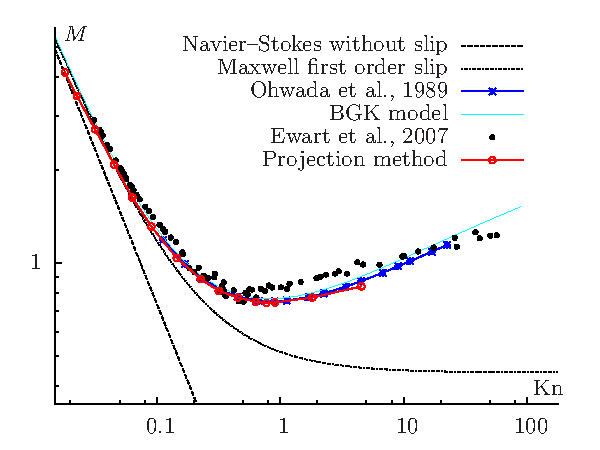
\includegraphics[width=0.5\textwidth]{poiseuille}
	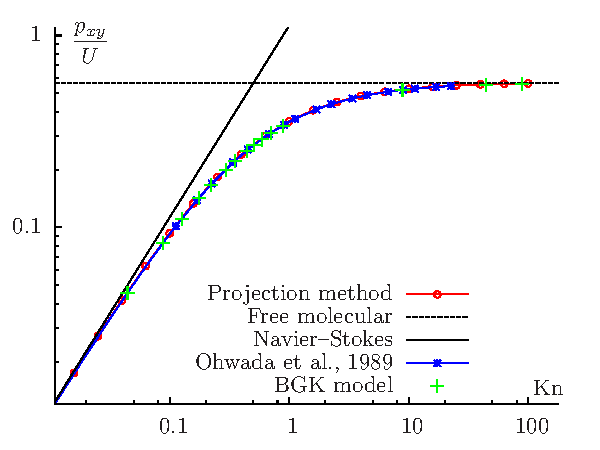
\includegraphics[width=0.5\textwidth]{couette}
	\caption{Безразмерные поток массы \(M\) для задачи Пуазёйля и сдвиговое напряжение \(p_{xy}\) 
		для задачи Куэтта в зависимости от числа Кнудсена \(\mathrm{Kn}\).}\label{fig}
\end{figure}

Впервые с помощью численных методов рассматриваемые задачи в линейном приближении (малые градиенты макропараметров)
были точно решены для молекулярной модели твёрдых сфер группой японских учёных из Киотского университета~\cite{Ohwada1989, Sone1990}.
Ранее физическое описание этих задач ограничивалось модельными уравнениями.
Непосредственные эксперименты протекания водорода через стеклянные каналы проводятся до сих пор~\cite{Ewart2007},
поскольку получение высокой точности измерений разреженного газа --- достаточно сложная техническая задача.
На рис.~\ref{fig} представлены некоторые результаты, полученные различными методами.
Газ в обоих задачах заключён между двумя бесконечными параллельными пластинами.  

Однако цель нашего рассмотрения упомянутых классических течений --- это верификация численного метода,
который может быть применён для широкого класса задач разреженного газа.
Речь идёт о консервативной конечно-разностной схеме решения уравнения Больцмана
на основе проекционного метода дискретных ординат для вычисления интеграла столкновений~\cite{Tcheremissine1997}.
Подробное описание программной реализации можно найти в~\cite{Our2011}.

Результатом проведённого исследования является демонстрация хорошей сходимости численного моделирования к эталонным табличным значениям,
особенно в переходном режиме, т.е. для чисел Кнудсена порядка единицы. Этот диапазон традиционно считается проблематичным
как для асимптотических методов решения, так и для статистических (DSMC).
Кроме того, экспериментально показан второй порядок сходимости по отношению к шагу равномерной шарообразной разностной сетки в пространстве скоростей.

\begin{thebibliography}{9}
\bibitem{Ohwada1989}
	T. Ohwada, Y. Sone, K. Aoki. Numerical analysis of the Poiseuille and thermal transpiration flows between two parallel plates on the basis of the Boltzmann equation for hard-sphere molecules.
	{\it Physics of Fluids A: Fluid Dynamics},
	1(12):~2042--2049, 1989.
\bibitem{Sone1990}
	Y. Sone, S. Takata, T. Ohwada. Numerical analysis of the plane Couette flow of a rarefied gas on
	the basis of the linearized Boltzmann equation for hard-sphere molecules.
	{\it European Journal of Mechanics B Fluids},
	9:~273--288, 1990.
\bibitem{Ewart2007}
	T. Ewart et al. Mass flow rate measurements in a microchannel, from hydrodynamic
	to near free molecular regimes.
	{\it Journal of Fluid Mechanics},
	584:~337--356, 2007.
\bibitem{Tcheremissine1997}
	Черемисин Ф.Г. Консервативный метод вычисления интеграла столкновений Больцмана.
	{\it Доклады РАН},
	357(1):~53--56, 1997.
\bibitem{Our2011}
	Додулад О.И., Клосс Ю.Ю., Мартынов Д.В., Рогозин О.А., Рябченков В.В., Черемисин Ф.Г., Шувалов П.В.
	Проблемно-моделирующая среда для расчётов и анализа газокинетических процессов.
	{\it Нано- и микросистемная техника},
	2:~12--17, 2011.

\end{thebibliography}

\end{document}
